% **************************************************
% Clean Thesis
% -- A LaTeX Style for Thesis Documents --
% 
% Copyright (C) 2011-2014 Ricardo Langner
% **************************************************
%
% Readme:
% ----------------------------------------
% *** Clean, Simple, Elegant ***
% "Clean Thesis" is a LaTeX style for thesis documents, developed
% for my diplom thesis (Diplomarbeit). The style can be understood
% as my personal compromise - a typical clean looking scientific
% document combined and polished with minor beautifications.
% 
% The design of this "Clean Thesis" style is inspired
% by user guide documents from Apple Inc.
% 
% Note: If you are looking for an exact and correct style regarding
% typographic rules, please have a look at the "Classic Thesis Style"
% (see http://www.miede.de/index.php?page=classicthesis).
% 
% *** Donation = Postcard ***
% Based on the idea of Andr\'e Miede: If you like the "Clean Thesis"
% style I would be very pleased about a donation in the form of a
% POSTCARD. You can find my address in the file Clean-Thesis.pdf.
% I am going to collect all postcards and exhibit them at the website
% I mentioned.
% 
% *** Idea and Inspiration ***
% The idea of providing my customized style for thesis documents
% passed through my mind while writing my own thesis. Motivated and
% inspired by the superb "Classic Thesis Style"
% (see http://www.miede.de/index.php?page=classicthesis) by Andr\'e Miede
% (thanks to Andr\'e for doing a great job) I decided to collect all
% design and style related functionality in a separate LaTeX style and
% provide this style to other thesis writers.
% 
% 
% License Information:
% ----------------------------------------
% "Clean Thesis" is free software: you can redistribute it and/or modify
% it under the terms of the GNU General Public License as published by
% the Free Software Foundation, either version 3 of the License, or
% (at your option) any later version.
% 
% "Clean Thesis" is distributed in the hope that it will be useful,
% but WITHOUT ANY WARRANTY; without even the implied warranty of
% MERCHANTABILITY or FITNESS FOR A PARTICULAR PURPOSE.  See the
% GNU General Public License for more details.
% 
% You should have received a copy of the GNU General Public License
% along with this program.  If not, see <http://www.gnu.org/licenses/>.
% **************************************************


% **************************************************
% Document Class Definition
% **************************************************
\documentclass[%
	paper=A4,					% paper size --> A4 is default in Germany
	twoside=true,				% onesite or twoside printing
	openright,					% doublepage cleaning ends up right side
	parskip=full,				% spacing value / method for paragraphs
	chapterprefix=true,		% prefix for chapter marks
	11pt,							% font size
	headings=normal,		% size of headings
	bibliography=totoc,		% include bib in toc
	listof=totoc,					% include listof entries in toc
	titlepage=on,				% own page for each title page
	captions=tableabove,	% display table captions above the float env
	draft=false,					% value for draft version
]{scrreprt}%

% **************************************************
% Debug LaTeX Information
% **************************************************
%\listfiles

% **************************************************
% Information and Commands for Reuse
% **************************************************
\newcommand{\thesisTitle}{Individualized feedback for lexical stress errors}
\newcommand{\thesisSubtitle}{Towards a CAPT system for French learners of German}

\newcommand{\authorName}{Anjana Sofia Vakil}
\newcommand{\authorContact}{anjanav@coli.uni-saarland.de}

\newcommand{\thesisSubject}{Thesis subject (whatever that means)}
\newcommand{\thesisDate}{10 Never, 2014}
%\newcommand{\thesisVersion}{Thesis version (what is this?)}

%\newcommand{\thesisFirstReviewer}{Jane Doe}
%\newcommand{\thesisFirstReviewerUniversity}{\protect{Clean Thesis Style University}}
%\newcommand{\thesisFirstReviewerDepartment}{Department of Clean Thesis Style}
%
%\newcommand{\thesisSecondReviewer}{John Doe}
%\newcommand{\thesisSecondReviewerUniversity}{\protect{Clean Thesis Style University}}
%\newcommand{\thesisSecondReviewerDepartment}{Department of Clean Thesis Style}

\newcommand{\thesisFirstSupervisor}{Prof. Dr. Bernd M\"{o}bius}
\newcommand{\thesisSecondSupervisor}{Dr. J\"{u}rgen Trouvain}

\newcommand{\thesisUniversity}{\protect{Saarland University}}
\newcommand{\thesisUniversityDepartment}{Department of Computational Linguistics \& Phonetics}
\newcommand{\thesisUniversityInstitute}{Fachrichtung 4.7 Allgemeine Linguistik
}
%\newcommand{\thesisUniversityGroup}{Clean Thesis Group (CTG)}
\newcommand{\thesisUniversityCity}{Saarbr\"{u}cken}
\newcommand{\thesisUniversityStreetAddress}{Postfach 15 11 50}
\newcommand{\thesisUniversityPostalCode}{66041}

% **************************************************
% Load and Configure Packages
% **************************************************
\usepackage[utf8]{inputenc}		% defines file's character encoding
\usepackage[english]{babel} % babel system, adjust the language of the content
\usepackage[					% clean thesis style
	figuresep=colon,%
	sansserif=false,%
	hangfigurecaption=false,%
	hangsection=true,%
	hangsubsection=true,%
	colorize=full,%
	colortheme=bluemagenta,%
]{cleanthesis}

\hypersetup{					% setup the hyperref-package options
	pdftitle={\thesisTitle},	% 	- title (PDF meta)
	pdfsubject={\thesisSubject},% 	- subject (PDF meta)
	pdfauthor={\authorName},	% 	- author (PDF meta)
	plainpages=false,			% 	- 
	colorlinks=false,			% 	- colorize links?
	pdfborder={0 0 0},			% 	-
	breaklinks=true,			% 	- allow line break inside links
	bookmarksnumbered=true,		%
	bookmarksopen=true			%
}

%TODO reverse in final version
\DeclareGraphicsExtensions{.png,.pdf}

\addbibresource{library.bib}

% **************************************************
% Document CONTENT
% **************************************************
\begin{document}

% --------------------------
% rename document parts
% --------------------------
%\renewcaptionname{ngerman}{\figurename}{Abb.}
%\renewcaptionname{ngerman}{\tablename}{Tab.}
\renewcaptionname{english}{\figurename}{Fig.}
\renewcaptionname{english}{\tablename}{Tab.}

% --------------------------
% Front matter
% --------------------------
\pagenumbering{roman}			% roman page numbing (invisible for empty page style)

\pagestyle{empty}					% no header or footers
% !TEX root = ../thesis-example.tex
%
% ------------------------------------  --> cover title page
\begin{titlepage}
	\pdfbookmark[0]{Cover}{Cover}
	\tgherosfont
	\flushright
	\hfill
	\vfill
	
	{\color{ctcolormain}
	{\LARGE\textbf{\thesisTitle}} \par
	{\Large \thesisSubtitle} \par
	} %end coloring
	
	\rule[5pt]{\textwidth}{.4pt} \par
	
	{\LARGE \authorName} \\[2mm]
%TODO include email here?  		\texttt{\authorContact}

	\vfill
	
	
	\textit{A thesis submitted toward the degree of} \\[1mm]
	{\Large Master of Science} \\[1mm]
	{\large in Language Science and Technology} \\	
	
	\vfill	
	
	\textit{Prepared under the supervision of} \\
	\thesisFirstSupervisor \\
	\thesisSecondSupervisor 
	
	\vfill
	
	
	%
\includegraphics[width=6cm]{img/uni_des_saarlandes} \\[2mm]
	{\Large \thesisUniversity} \\[2mm]
	{\large \thesisUniversityDepartment} \\
	%{\large \thesisUniversityInstitute \\}
	
	\vfill
	
	\thesisDate \\
	
\end{titlepage}


% ------------------------------------  --> lower title back for single page layout
\hfill
\vfill
\small
%TODO copyright?
{\tgherosfont \textbf{\authorName}} \\
\texttt{\authorContact}\\
\textit{\thesisTitle} \\
%\thesisSubject, 
\thesisDate \\
Supervisors: \thesisFirstSupervisor\ and \thesisSecondSupervisor \\

{\tgherosfont \textbf{\thesisUniversity}} \\
%\textit{\thesisUniversityGroup} \\
\thesisUniversityDepartment \\
\thesisUniversityInstitute \\
\thesisUniversityStreetAddress \\
\thesisUniversityPostalCode\ and \thesisUniversityCity \\[1.5em]

Typeset using \LaTeXe.
Style adapted from the \textit{Clean Thesis} template developed by Ricardo Langner (\url{http://cleanthesis.der-ric.de/}).
	% INCLUDE: all titlepages
\cleardoublepage

\pagestyle{empty}					% no header or footers
% !TEX root = ../thesis-example.tex
%
%************************************************
% Declaration
%************************************************
\pdfbookmark[0]{Declaration}{Declaration}
\chapter*{Declaration}
\label{sec:declaration}
\thispagestyle{empty}

%I hereby declare that this thesis, presented here toward the completion of the Master of Science degree, is my own original work. All material contained herein that has been taken from other sources is acknowledged as such, without exception.

%\smallskip

%\noindent\textit{\thesisUniversityCity, \thesisDate}

%\begin{flushright}
%	\begin{minipage}{5cm}
%		\rule{\textwidth}{1pt}
%		\centering\authorName
%	\end{minipage}
%\end{flushright}

\textbf{Eidesstattliche Erklärung}

Hiermit erkläre ich, dass ich die vorliegende Arbeit selbstständig verfasst und keine anderen als die angegebenen Quellen und Hilfsmittel verwendet habe.

\smallskip

\textbf{Declaration}

I hereby confirm that the thesis presented here is my own work, with all assistance acknowledged.

\bigskip

\begin{flushright}
\noindent\textit{\thesisUniversityCity, \thesisDate}

\bigskip

\rule{5cm}{1pt}

\authorName
\end{flushright}





%*****************************************
%*****************************************
	% INCLUDE: all titlepages
\cleardoublepage

\pagestyle{plain}						% display just page numbers
% !TEX root = Clean-Thesis.tex
%
\pdfbookmark[0]{Abstract}{Abstract}
\chapter*{Abstract}
\label{sec:abstract}
\vspace*{-10mm}

The prosodic realization of lexical stress, the phenomenon by which certain syllable(s) in a word are accentuated more than others, is an important feature of the German phonological system, but one that can pose a considerable challenge to students learning German as a foreign language (L2). This challenge is particularly daunting for native (L1) speakers of French, as lexical stress is realized quite differently (or perhaps not at all) in French word prosody.
As pronunciation training typically demands substantial individual attention from an instructor, which is not always feasible in classroom language-learning settings, Computer Assisted Pronunciation Training (CAPT) has emerged over recent decades as a promising way of using technology to deliver individualized pronunciation training in the absence of a human teacher.
This thesis investigates how CAPT can be used to help L1 French speakers learning German as L2 improve their pronunciation with regard to lexical stress prosody.

%First, i
In an effort to illuminate the nature of L1 French learners' lexical stress errors in German, the thesis 
describes the manual annotation of lexical stress errors in a learner speech corpus,
and presents an analysis of the frequency and types of errors observed.
%presents an analysis of the frequency and types of errors observed in a learner speech corpus manually annotated for lexical stress errors.
A variety of methods for automatically diagnosing such errors in learner word utterances are then explored, including novel methods for diagnosis by means of classification using supervised machine learning, as well as by means of comparison with one or more reference utterances, i.e. the same word pronounced by a native German speaker.
The ways in which diagnoses produced by these methods can be used to deliver diverse types of feedback on these errors are then explored, including types which have not previously been utilized in German CAPT. 

In its most important contribution, this thesis describes the development of a prototype CAPT tool %, \TODO{de-stress},
%: German (deutsche) System for Training and Research on Errors in Second-language Stress, 
which integrates these various diagnostic and feedback methods via an easy-to-use web interface. 
%a system for use by language learners and teachers as well as researchers of language acquisition
This tool is designed not only to provide students with feedback on their lexical stress errors, but also to facilitate research on the efficacy of the various
% diagnostic and feedback methods 
 types of diagnosis and feedback
 explored in this thesis, and to enable L2 German teachers 
 %to choose from these methods 
 to create exercises best suited to their students' needs; it thus constitutes an important step towards the development of a comprehensive, intelligent CAPT system for French learners of German. 




%\vspace*{20mm}
%
%%{\usekomafont{chapter}Abstract (different language)}\label{sec:abstract-diff} \\
%%
%%\blindtext
		% INCLUDE: the abstract
\cleardoublepage
%
% !TEX root = ../thesis-example.tex
%
\pdfbookmark[0]{Acknowledgments}{Acknowledgments}
\chapter*{Acknowledgments}
\label{sec:thanks}
\vspace*{-10mm}


First of all, I am extremely grateful to my thesis supervisors at {\thesisUniversity}, \textbf{Prof. Dr. Bernd Möbius} and \textbf{Dr. Jürgen Trouvain}; this thesis could not have been written without their support, encouragement, and feedback.

The work reported in this thesis was partially supported by the Franco-German project \textit{Individualized Feedback for Computer-Assisted Spoken Language learning} (IFCASL), funded jointly by the Deutsche Forschungsgemeinschaft (DFG) and the Agence Nationale de la Recherche (ANR). I thank the the entire \textbf{Project IFCASL team} at both Saarland University (Saarbrücken, Germany) and LORIA (Nancy, France) for giving me the opportunity to work with them on this project over the last two years, and for supporting my work at both institutions.

Among the researchers at LORIA, I would especially like to thank:
\textbf{Dr. Yves Laprie} for providing invaluable information on the automatic processing of prosody and for generously sharing his office with me;
\textbf{Dr. Julie Busset} for allowing me to work closely with her on refactoring the \textit{JSnoori} software to facilitate integration with programs such as \textit{de-stress};
\textbf{Dr. Anne Bonneau} for advising me on feedback on prosody in nonnative speech and for welcoming me in Nancy;
%prosody feedback in Computer-Assisted Language Learning (CAPT);
and 
\textbf{Dr. Dominique Fohr} and \textbf{Dr. Odile Mella} for elucidating the automatic segmentation of nonnative speech. 
%Dr. Julie Busset, Dr. Vincent Colotte,  and Dr. Yves Laprie 
%at LORIA, who provided invaluable advice on prosody in Computer-Assisted Language Learning (CAPT), speech processing, and integration of the \textit{JSnoori} software with the \textit{de-stress} system. 

I am also extremely grateful to IFCASL team members \textbf{Jeanin Jügler} and \textbf{Dr. Frank Zimmerer} at {\thesisUniversity} for all their help, and especially for assisting with the lexical stress error annotation project and providing the German translation of the thesis abstract. 

I would additionally like to thank the \textbf{annotators} (not named to preserve anonymity) who donated their time to the error annotation project; without the labeled data produced through their efforts, much of the work reported in this thesis would not have been possible.

My heartfelt thanks also go to \textbf{Marie Springinsfeld} for generously providing the French translation of the thesis abstract, and to \textbf{Max Rabkin} and \textbf{Nathaneil Ward} for kindly helping to proofread this document.

Finally, I would like to express my gratitude to 
my mother, \textbf{Eileen Julian}, and to {my wonderful friends} in Saarbrücken and around the world.
%my friends and family, 
%especially Eileen Julian, James Newman, Max Rabkin, Rebecca Row, and Nat Ward, 
I could not have completed this thesis or the studies leading up to it without 
their loving support. % INCLUDE: acknowledgement
\cleardoublepage
%
%\setcounter{tocdepth}{2}		% define depth of toc
\tableofcontents					% display table of contents
\cleardoublepage

\listoffigures
\cleardoublepage

\listoftables
\cleardoublepage


% --------------------------
% Body matter
% --------------------------
\pagenumbering{arabic}			% arabic page numbering
\setcounter{page}{1}			% set page counter
\pagestyle{maincontentstyle} 	% fancy header and footer

% !TEX root = ../thesis-example.tex
%
\chapter{Introduction}
\label{chap:intro}

%\cleanchapterquote{You can’t do better design with a computer, but you can speed up your work enormously.}{Wim Crouwel}{(Graphic designer and typographer)}

\blindtext \parencite{Duong2011}.

\citeauthor{Sitaram2011} (\citeyear{Sitaram2011}) says blah blah blah.

\begin{table}
\caption{I made a table, isn't that awesome?}
\begin{tabular}{lll}
some & stuff & in \\
a & pretty & table \\
\end{tabular}
\end{table}


\section{Motivation and Problem Statement}
\label{sec:intro:motivation}

\Blindtext[3][1]

\section{Results}
\label{sec:intro:results}

\Blindtext[1][2]

\chapter{Proposed Thesis Structure}
\label{chap:structure}
\blindtext 

\section{Background and related work}
\blindtext

\subsection{CAPT and the IFCASL project}
\blindtext

\subsection{Error types/which errors to address}
\blindtext

\begin{figure}[htb]
	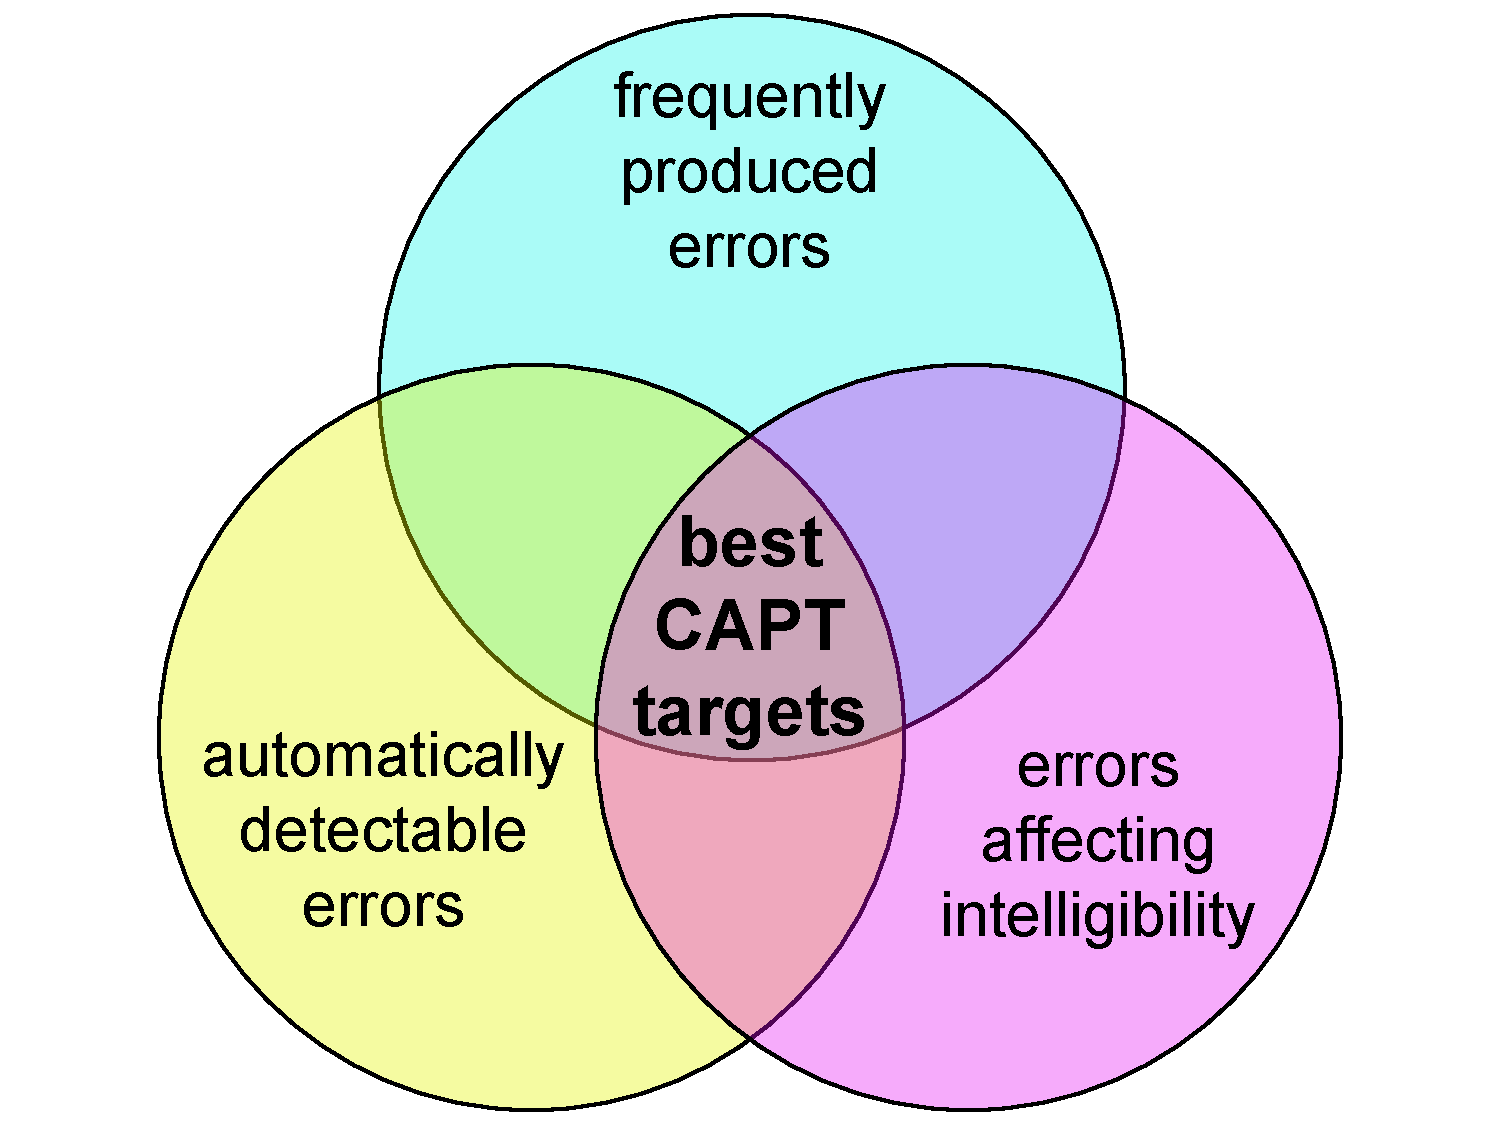
\includegraphics[width=\textwidth]{../img/error-venn}
	\caption{Criteria for determining which errors to address in a CAPT system.}
	\label{fig:errors}
\end{figure}

\paragraph{Lexical stress/Prosody in German and French}
\blindtext

\subsection{Prosody feedback in CAPT}
\blindtext

\section{Diagnosis}
\blindtext

\section{Feedback}
\blindtext

\begin{figure}[htb]
	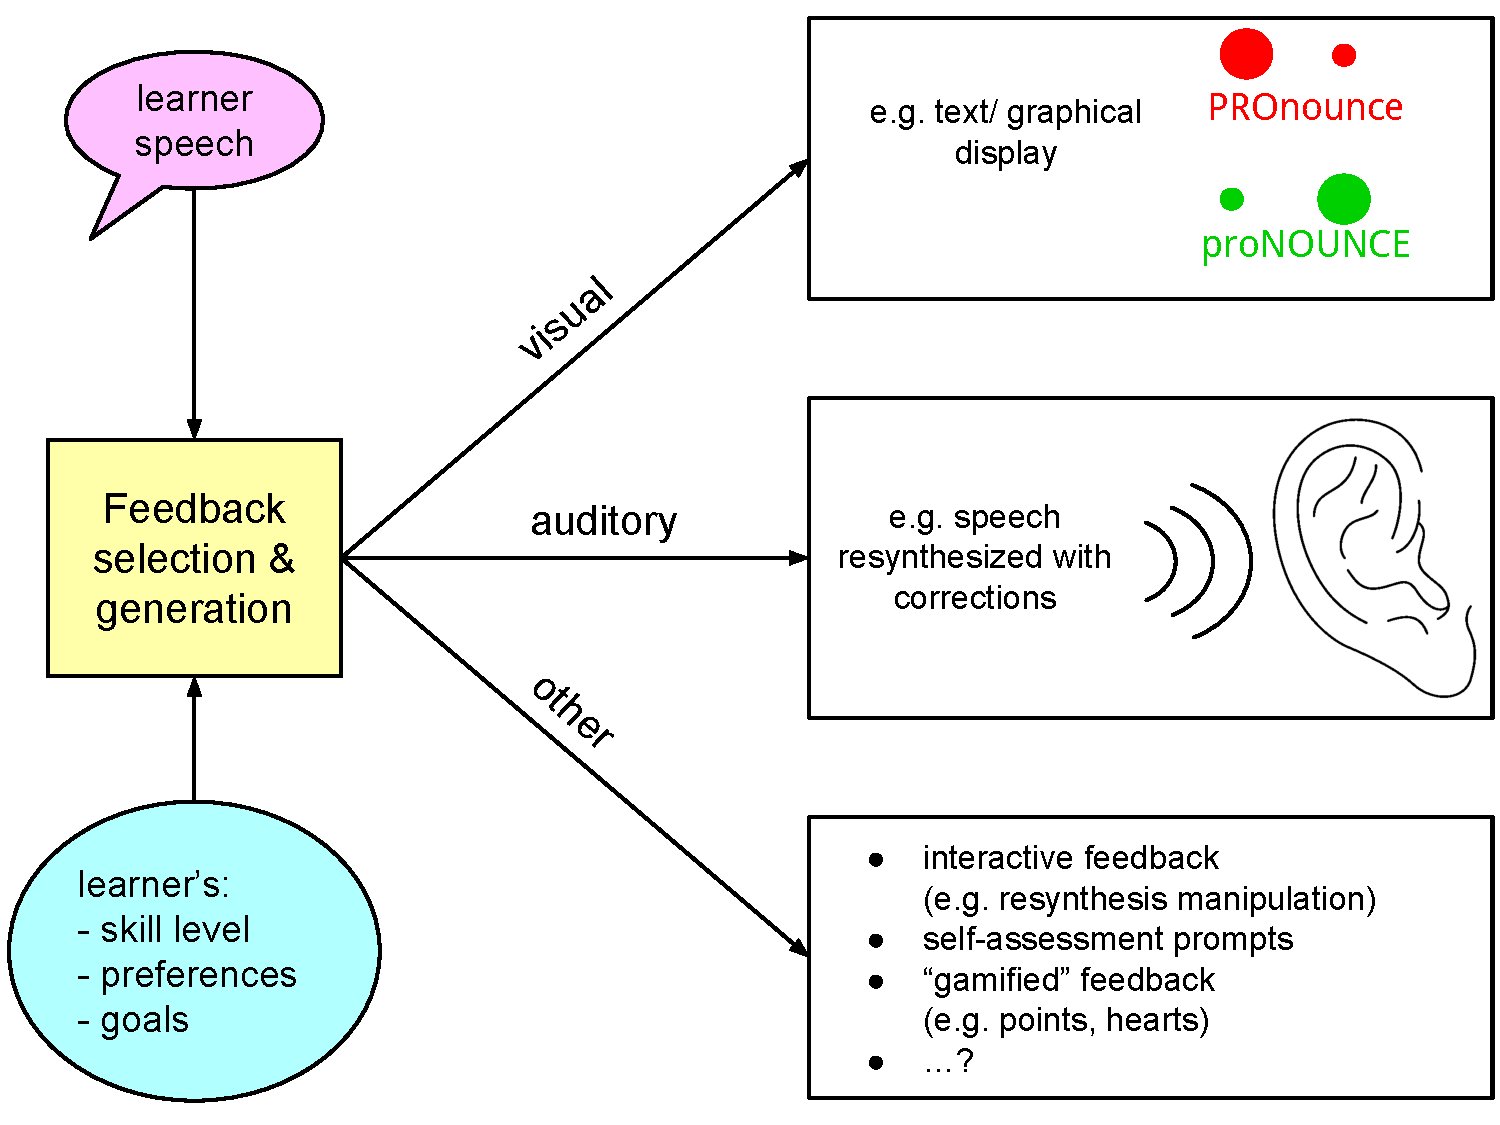
\includegraphics[width=\textwidth]{../img/feedback}
	\caption{Delivery of prosody feedback in different modalities.}
	\label{fig:feedback}
\end{figure}


\section{Future work}
\blindtext

\section{Conclusion}
\blindtext

%\textbf{Chapter \ref{sec:related}} \\[0.2em]
%\blindtext
%
%\textbf{Chapter \ref{sec:system}} \\[0.2em]
%\blindtext
%
%\textbf{Chapter \ref{sec:concepts}} \\[0.2em]
%\blindtext
%
%\textbf{Chapter \ref{sec:concepts}} \\[0.2em]
%\blindtext
%
%\textbf{Chapter \ref{sec:conclusion}} \\[0.2em]
%\blindtext


%% !TEX root = ../thesis-example.tex
%
\chapter{Introduction}
\label{sec:intro}

\cleanchapterquote{You can’t do better design with a computer, but you can speed up your work enormously.}{Wim Crouwel}{(Graphic designer and typographer)}

\Blindtext[2][2]

\section{Postcards: My Address}
\label{sec:intro:address}

\textbf{Ricardo Langner} \\
Alfred-Schrapel-Str. 7 \\
01307 Dresden \\
Germany


\section{Motivation and Problem Statement}
\label{sec:intro:motivation}

\Blindtext[3][1]

\section{Results}
\label{sec:intro:results}

\Blindtext[1][2]

\section{Thesis Structure}
\label{sec:intro:structure}

\textbf{Chapter \ref{sec:related}} \\[0.2em]
\blindtext

\textbf{Chapter \ref{sec:system}} \\[0.2em]
\blindtext

\textbf{Chapter \ref{sec:concepts}} \\[0.2em]
\blindtext

\textbf{Chapter \ref{sec:concepts}} \\[0.2em]
\blindtext

\textbf{Chapter \ref{sec:conclusion}} \\[0.2em]
\blindtext
 % INCLUDE: introduction
%% !TEX root = ../thesis-example.tex
%
\chapter{Related Work}
\label{sec:related}

\cleanchapterquote{A picture is worth a thousand words. An interface is worth a thousand pictures.}{Ben Shneiderman}{(Professor for Computer Science)}

\Blindtext[2][1]

\section{Related Work Section 1}
\label{sec:related:sec1}

\Blindtext[2][2]

\section{Related Work Section 2}
\label{sec:related:sec2}

\Blindtext[3][2]

\section{Related Work Section 3}
\label{sec:related:sec3}

\Blindtext[4][2]

\section{Conclusion}
\label{sec:related:conclusion}

\Blindtext[2][1]
 % INCLUDE: related work
% !TEX root = ../thesis-example.tex
%
\chapter{System}
\label{sec:system}

\cleanchapterquote{Innovation distinguishes between a leader and a follower.}{Steve Jobs}{(CEO Apple Inc.)}

\Blindtext[2][1]

\section{System Section 1}
\label{sec:system:sec1}

\Blindtext[1][2]

\begin{figure}[htb]
	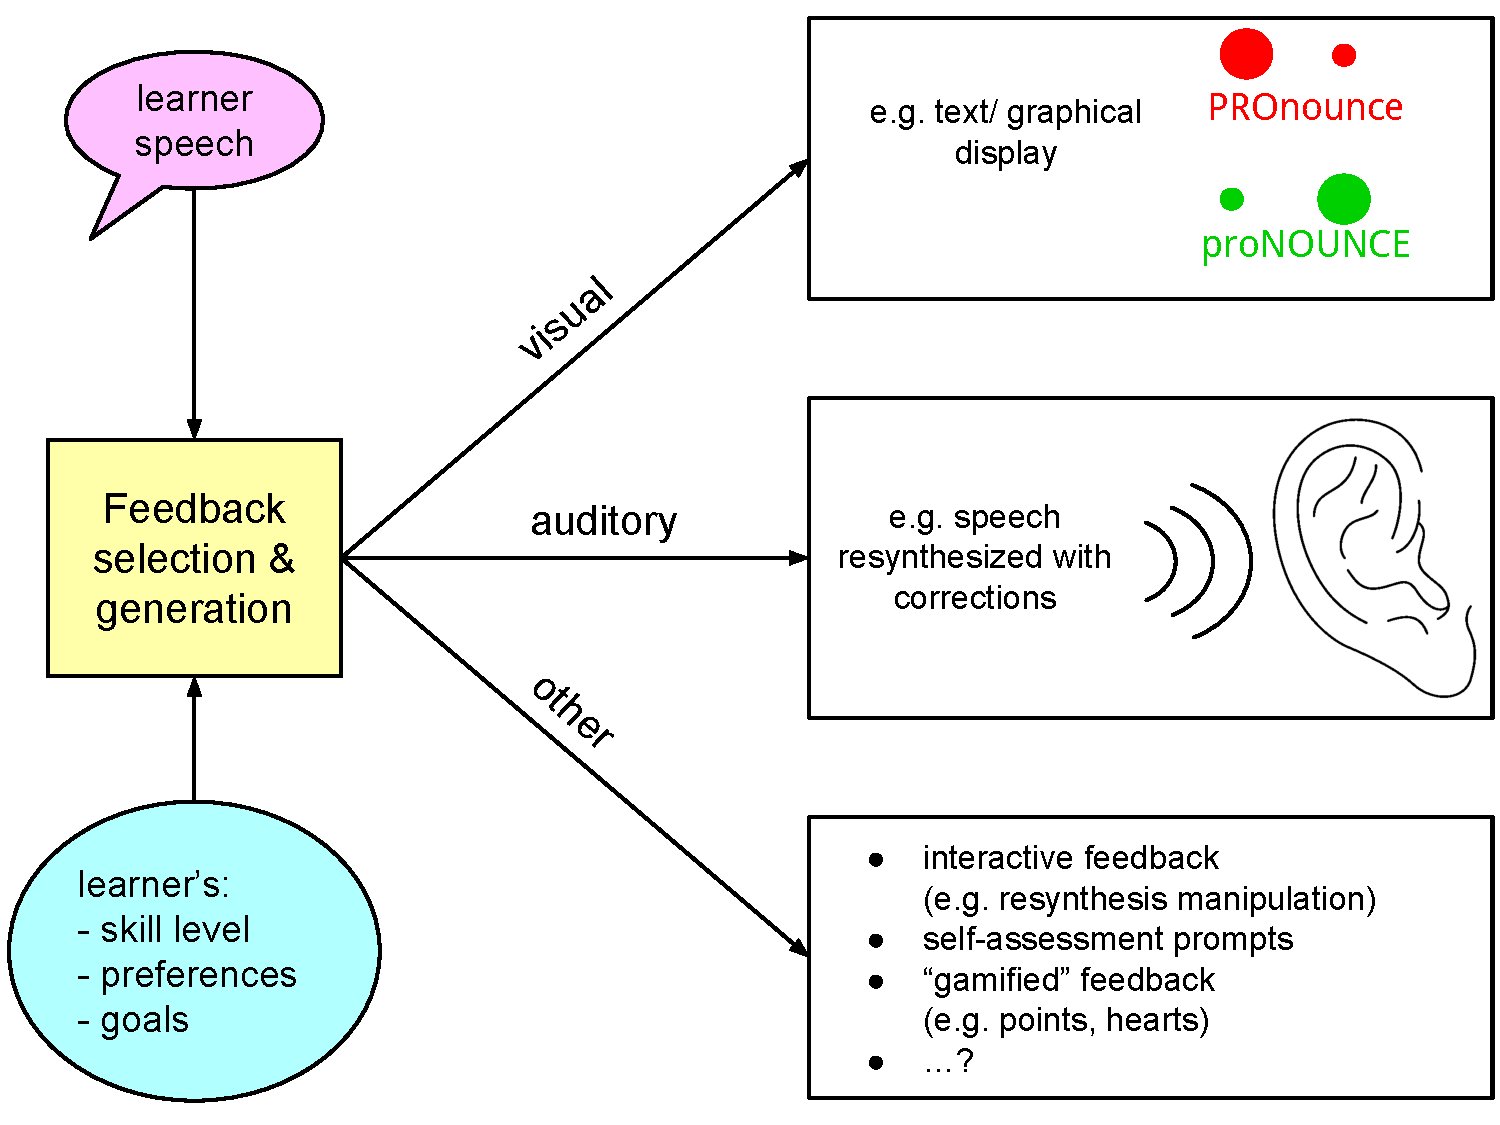
\includegraphics[width=\textwidth]{../img/feedback}
	\caption{Figure example: \textit{(a)} example part one, \textit{(c)} example part two; \textit{(c)} example part three}
	\label{fig:system:example1}
\end{figure}

\Blindtext[1][2]

\section{System Section 2}
\label{sec:system:sec2}

\Blindtext[1][2]

\begin{figure}[htb]
	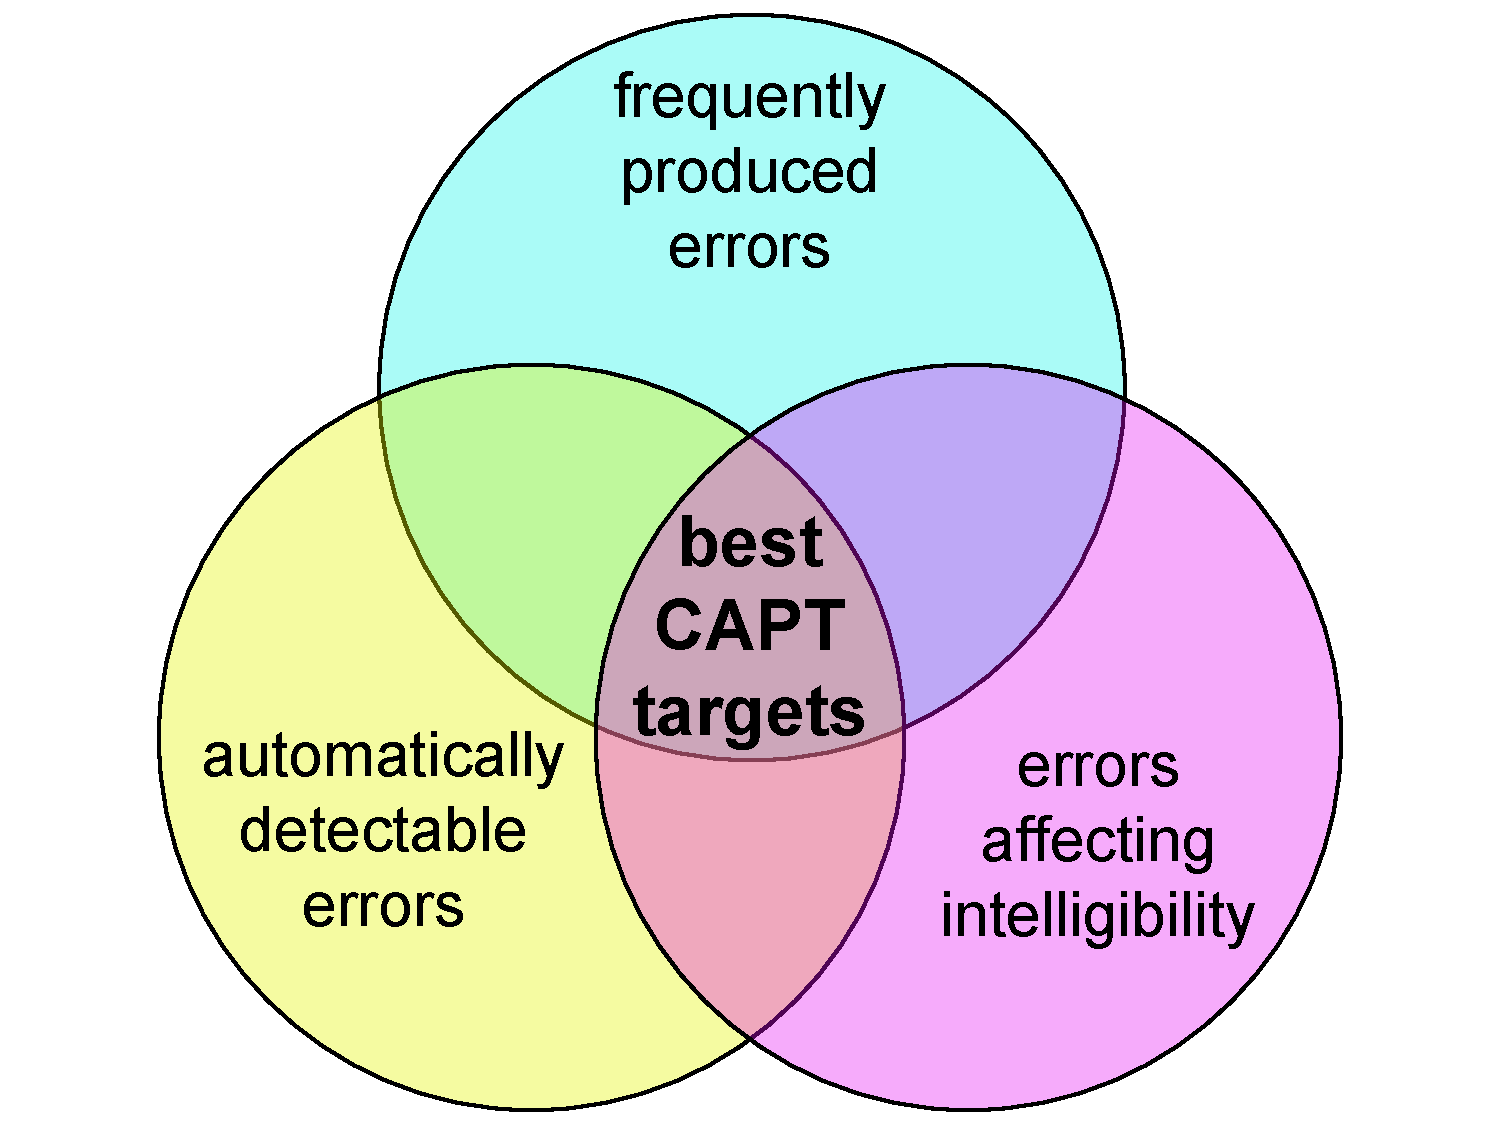
\includegraphics[width=\textwidth]{../img/error-venn}
	\caption{Another Figure example: \textit{(a)} example part one, \textit{(c)} example part two; \textit{(c)} example part three}
	\label{fig:system:example2}
\end{figure}

\Blindtext[2][2]

\section{System Section 3}
\label{sec:system:sec3}

\Blindtext[4][2]

\section{Conclusion}
\label{sec:system:conclusion}

\Blindtext[2][1]
	% INCLUDE: system
%% !TEX root = ../thesis-example.tex
%
\chapter{Concepts: This text is here to test a very long title, to simulate the line break behavior, to show that an extremely long tilte also works}
\label{sec:concepts}

\cleanchapterquote{Users do not care about what is inside the box, as long as the box does what they need done.}{Jef Raskin}{about Human Computer Interfaces}

\Blindtext[2][1]

\section{Concepts Section 1}
\label{sec:concepts:sec1}

\Blindtext[2][2]

\section{Concepts Section 2}
\label{sec:concepts:sec2}

\Blindtext[3][2]

\section{Concepts Section 3}
\label{sec:concepts:sec3}

\Blindtext[4][2]

\section{Conclusion}
\label{sec:concepts:conclusion}

\Blindtext[2][1]
 % INCLUDE: concepts
%% !TEX root = ../thesis-example.tex
%
\chapter{Conclusion}
\label{sec:conclusion}

\Blindtext[2][1]

\section{System Section 1}
\label{sec:conclusion:sec1}

\Blindtext[2][2]

\section{System Section 2}
\label{sec:conclusion:sec2}

\Blindtext[3][2]

\section{Future Work}
\label{sec:conclusion:future}

\Blindtext[2][2]
 % INCLUDE: conclusion
\cleardoublepage

% --------------------------
% Back matter
% --------------------------
{%
\setstretch{1.1}
\renewcommand{\bibfont}{\normalfont\small}
\setlength{\biblabelsep}{0pt}
\setlength{\bibitemsep}{0.5\baselineskip plus 0.5\baselineskip}
%\nocite{*}
\printbibliography%[title={References}]
%\printbibliography[nottype=online]
%\printbibliography[heading=subbibliography,title={Webseiten},type=online,prefixnumbers={@}]
}

\cleardoublepage
%
%\listoffigures
%\cleardoublepage
%
%\listoftables
%\cleardoublepage
%
%% !TEX root = ../thesis-example.tex
%
\pagestyle{empty}
\hfill
\vfill
\pdfbookmark[0]{Colophon}{Colophon}
\section*{Colophon}

This thesis was typeset with \LaTeXe.
It uses the \textit{Clean Thesis} style developed by Ricardo Langner.
The design of the \textit{Clean Thesis} style is inspired by user guide documents from Apple Inc.

Download the \textit{Clean Thesis} style at \url{http://cleanthesis.der-ric.de/}.

%\cleardoublepage
%
%% !TEX root = ../thesis-example.tex
%
%************************************************
% Declaration
%************************************************
\pdfbookmark[0]{Declaration}{Declaration}
\chapter*{Declaration}
\label{sec:declaration}
\thispagestyle{empty}

I hereby declare that this thesis, presented here toward the completion of the Master of Science degree, is my own original work. All material contained herein that has been taken from other sources is acknowledged as such, without exception.

\bigskip

\noindent\textit{\thesisUniversityCity, \thesisDate}

\smallskip

\begin{flushright}
	\begin{minipage}{5cm}
		\rule{\textwidth}{1pt}
		\centering\authorName
	\end{minipage}
\end{flushright}

%*****************************************
%*****************************************


%TODO put this back in? (instead of the \cleardoublepage after bib)
%\clearpage
%\newpage
%\mbox{}

% **************************************************
% End of Document CONTENT
% **************************************************
\end{document}
